\documentclass[conference]{IEEEtran}
\usepackage{cite}
\usepackage{amsmath,amssymb}
\usepackage{graphicx}
\usepackage{booktabs}
\usepackage{url}
\usepackage{textcomp}
\usepackage[T1]{fontenc}
\graphicspath{{../figures/}}
\hyphenation{Conversation Mood-Lens}

\setlength{\textfloatsep}{8pt plus 2pt minus 2pt}
\setlength{\floatsep}{8pt plus 2pt minus 2pt}
\setlength{\intextsep}{8pt plus 2pt minus 2pt}
\setlength{\abovecaptionskip}{4pt}
\setlength{\belowcaptionskip}{3pt}

\begin{document}

\title{MoodLens: Facial Expression Recognition in Two Real-World Applications, a Mood Based Menu Recommender and Conversation Coach}

\author{\IEEEauthorblockN{Abhishek KS}
\IEEEauthorblockA{School of Computer Science \& Engineering\\
RV University\\
Bangalore, India\\
abhishekks.btech23@rvu.edu.in}
\and
\IEEEauthorblockN{Deepak Murthy}
\IEEEauthorblockA{School of Computer Science \& Engineering\\
RV University\\
Bangalore, India\\
deepakmurthy@rvu.edu.in}}

\maketitle

\begin{abstract}
Facial Expression Recognition (FER) systems are generally reported with high accuracy on cropped static datasets. However, this is rarely tested within a real-world scenario. The presence of poor quality webcam input, head movement and latency will cause a decrease in accuracy and cause flickering of the predicted label. This paper details MoodLens, an application based around a ResNet-18 classifier trained on the FER-2013 dataset and fine-tuned on the FER+ label distributions. This application was implemented in two separate web applications. In the first, Smash Guys Mood Menu, the application uses the facial expression of the diner to create a four-course meal from a 72-dish menu. Constraints are applied to ensure the menu adheres to their diet, allergens, spice and budget. A Table Mode is also included to allow multiple diners to use the application. The final feature is Mood Lift, rescan the diner to compare the positivity of their expressions before and after. The second application, Conversation Coach, analyses the expressions of the conversation partner. It can identify quick micro-expressions occurring between 140--650\,ms, analyse multiple faces in a room, score the sentences being said based on the listener's reaction, and provide a debrief after the session. Both applications have a chatbot within them using Groq. The current state of the application is added to the prompt. The classifier has an accuracy of 69.99\% on FER-2013 and 85.08\% on FER+. The checkpoint used within the application had an accuracy of 83.38\% on FER+. This was chosen as it had a better recall performance on the rare classes. The classification occurs on the server using 22.6\,ms per frame of an Apple M2. An exponential smoothing algorithm was used with a hysteresis rule to reduce label changes for consistent faces. The number of label changes was reduced from 14.2 to 0.1 per 10 seconds, with a median delay of 2.36\,s when the actual expression changed. No constraint violations were found in 3000 trials of the recommender. 28 automated tests were also performed with all passing. These tests were self-designed and limitations are discussed.
\end{abstract}

\begin{IEEEkeywords}
Facial Expression Recognition, FER-2013, FER+, ResNet, Affective Computing, Recommender Systems, Conversation Coach, Micro-Expressions, Edge AI, Grounded Chatbots.
\end{IEEEkeywords}

\section{Introduction}
Benchmarking datasets, such as FER-2013~\cite{goodfellow}, FER+~\cite{barsoum}, and AffectNet~\cite{mollahosseini} have helped improve facial expression recognition with consistent improvements on small cropped static images. However, real-world scenarios introduce new issues:
\begin{enumerate}
    \item \textbf{Noise from camera and pose.} Webcams introduce motion blurring, uneven lighting and lens distortion. The user will also be constantly moving their head causing jitters in detected face bounding boxes and landmarks.
    \item \textbf{Label flickering.} Each frame is classified individually, meaning the label is constantly changing from frame to frame. This means a user could be labelled as sad, angry and neutral in one second whilst having a neutral expression.
    \item \textbf{Not useful.} A vector such as ``happy 0.62, neutral 0.28'' would not be useful to the user. The application should provide a decision or advice from the vector.
    \item \textbf{Privacy and latency.} Sending the raw video stream to a remote server introduces latency and extra bandwidth. There are also clear privacy issues.
\end{enumerate}

These issues are overcome by detecting and classifying locally. The output is then sent through a temporal filter. Two applications were created, each run on its own FastAPI process:
\begin{itemize}
    \item \textbf{Smash Guys Mood Menu.} The system detects what mood the diner is in based on their expression. It then searches through a 72-dish menu to find a combination of four courses based on their dietary, allergen, spice and budget requirements. Once they have eaten, they can rescan and we can see how much their positivity has increased. This is then used to change the weights for future recommendations (Mood Lift).
    \item \textbf{Live Conversation Coach.} The system is pointed at the conversation partner or meeting. It gives a live positivity rating, identifies quick micro-expressions, identifies multiple faces in Room Mode, links the sentences said to the listener's reaction, and provides a debrief.
\end{itemize}

The video frames are processed locally using a WebSocket. Each application also contains a chatbot (Groq, gpt-oss-120b~\cite{gptoss}). The current menu, diner mood or conversation transcript is added to the system prompt so the chatbot can relate its answers to the actual application.

\section{Related Work}
\subsection{Datasets and Architectures}
Early FER systems used manually engineered features such as Gabor wavelets and Local Binary Patterns with Support Vector Machines~\cite{pantic}. FER-2013~\cite{goodfellow} became a standard benchmark with 7 classes (anger, disgust, fear, happiness, sadness, surprise, neutral). The images are small ($48\times48$px), have noisy labels and are unbalanced. The human accuracy is estimated to be approximately 65\% $\pm$ 5\%. FER+~\cite{barsoum} relabelled the images with 10 crowd annotators. This data was released with the vote distributions. A survey of the field is provided by Li and Deng~\cite{li}. They note there has been a shift towards using residual networks~\cite{he}, attention and self-supervised pre-training. A ResNet-18 network was used as the backbone. First trained on FER-2013 then fine-tuned on the Soft Labels of FER+.

\subsection{Affective Food Recommendation}
There is a bidirectional relationship between the affective state and eating behaviour. Macht~\cite{macht} describes 5 ways emotions can influence eating behaviour including motivation, sensory perception and food choice. Gibson~\cite{gibson} provides a review on how palatable food can affect stress related hormones. Previous affective recommenders have mostly used mood tags. We have considered this as a constrained selection problem, where the mood affinity score is maximised with hard constraints on dietary, allergen, spice and budget requirements.

\subsection{Emotion Modelling and Micro-Expressions}
Two main emotion modelling frameworks exist. Ekman and Friesen's basic emotions~\cite{ekman71} and Russell's circumplex model~\cite{russell}. This places emotion on a valence and arousal axis. Barrett et al.~\cite{barrett} argue that there is no reliable mapping from facial configuration to a single internal state. This is why this is presented as a behavioural cue in our interfaces. The micro-expression detection uses early observations from Haggard and Isaacs~\cite{haggard} and Ekman and Friesen~\cite{ekman69}. The duration of micro-expressions are reported by Yan et al.~\cite{yan}.

\subsection{Grounded Chatbots}
Language models can provide incorrect information regarding specialised topics~\cite{rag}. Both chatbots receive validated data from the application in the system prompt. This includes the dish ID's in the menu, allergen filters, current diner mood, and conversation transcript.

\section{Data and Problem Setup}
\subsection{Benchmark Datasets}
\begin{itemize}
    \item \textbf{FER-2013.} Contains 28,709 training images, 3,589 public test images and 3,589 private test images. All images are $48\times48$ grayscale. The classes are heavily imbalanced (Fig.~\ref{fig:dataset}). The happiness class has 7,215 training images (25.1\%). The disgust class only has 436 training images (1.5\%).
    \item \textbf{FER+.} Images from FER-2013 with 10 annotations per image. Non-face images, unknown labels and contempt were removed. This resulted in 35,272 images. 28,224 were used for training. 3,529 for validation (PublicTest). 3,519 were used for testing (PrivateTest). Each image had an average of 8.8 valid votes.
\end{itemize}

\begin{figure*}[!t]
\centering
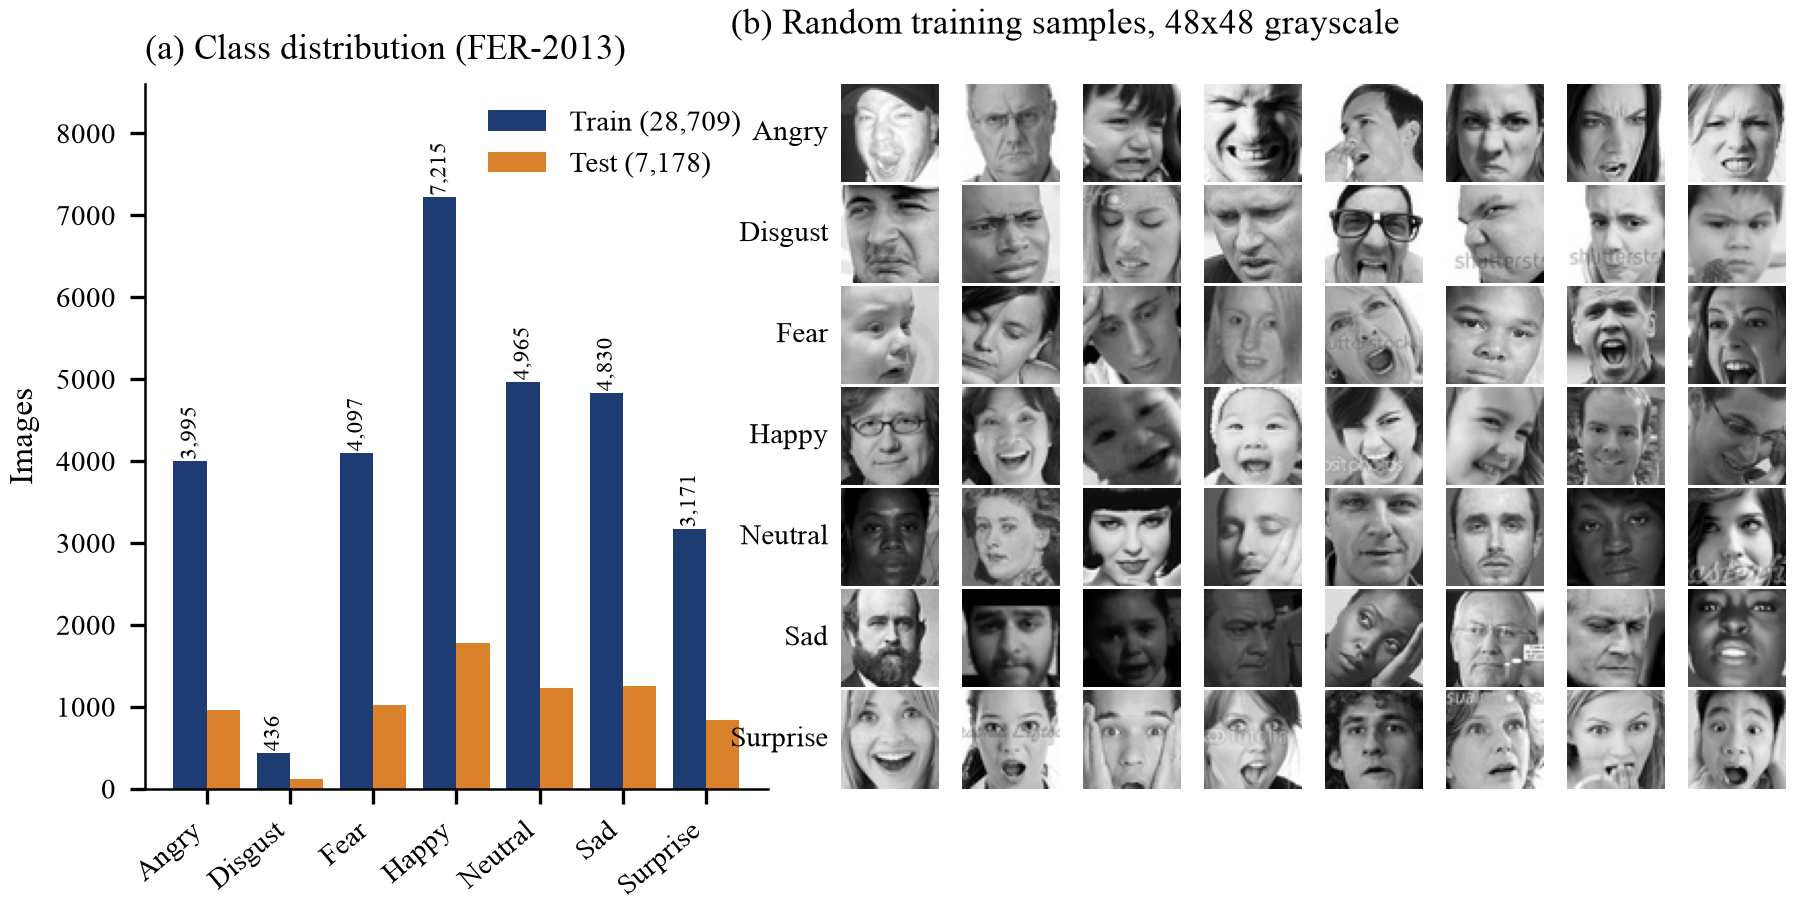
\includegraphics[width=0.88\textwidth]{fig_dataset.png}
\caption{FER-2013: (a) Imbalance of the classes between the 7 emotions. Only 436 samples for the disgust class. (b) Examples of training images ($48\times48$). Showing differences in lighting, pose, occlusion and ambiguous labels.}
\label{fig:dataset}
\end{figure*}

\begin{table}[!t]
\centering
\caption{Datasets and Knowledge Bases Used}
\label{tab:data}
\small
\begin{tabular}{@{}lrl@{}}
\toprule
Dataset / Corpus & Scale & Role \\
\midrule
FER-2013 Train & 28,709 & Stage 1 Training \\
FER-2013 Val Split & 2,868 & Hyperparameter selection \\
FER-2013 Test & 7,178 & Benchmarking \\
FER+ Train & 28,224 & Stage 2 Fine-Tuning \\
FER+ PrivateTest & 3,519 & Multi-Annotator Testing \\
Aligned FER Test & 6,970 & Camera Pipeline Testing \\
Restaurant Menu KB & 72 dishes & Recommender / Chatbot \\
Coaching Playbook & 35 scripts & Coach Advice \\
\bottomrule
\end{tabular}
\end{table}

\subsection{Knowledge Bases}
In addition to the image datasets, 2 knowledge bases were manually created (Table~\ref{tab:data}):
\begin{itemize}
    \item \textbf{Smash Guys Menu.} Contains 72 dishes split into 19 categories (29 Main, 11 Side, 28 Drink, 4 Dessert). Dishes are priced from \texttt{\_}130 to \texttt{\_}810. Each dish has 22 flavour descriptors (e.g. umami, spicy, refreshing, indulgent). The dish is either vegetarian or non-vegetarian. It has a spice rating (0 = mild, 1 = medium, 2 = hot). And contains allergen tags (egg, dairy, nuts, mushroom, alcohol).
    \item \textbf{Coaching Playbook.} Contains 35 scripts. Each emotion (7) has a script for each setting (5). Each script contains a brief description of the behaviour, suggested pace of voice, 3 things to do, 2 things to avoid, and 2 example phrases.
\end{itemize}

\begin{figure*}[!t]
\centering
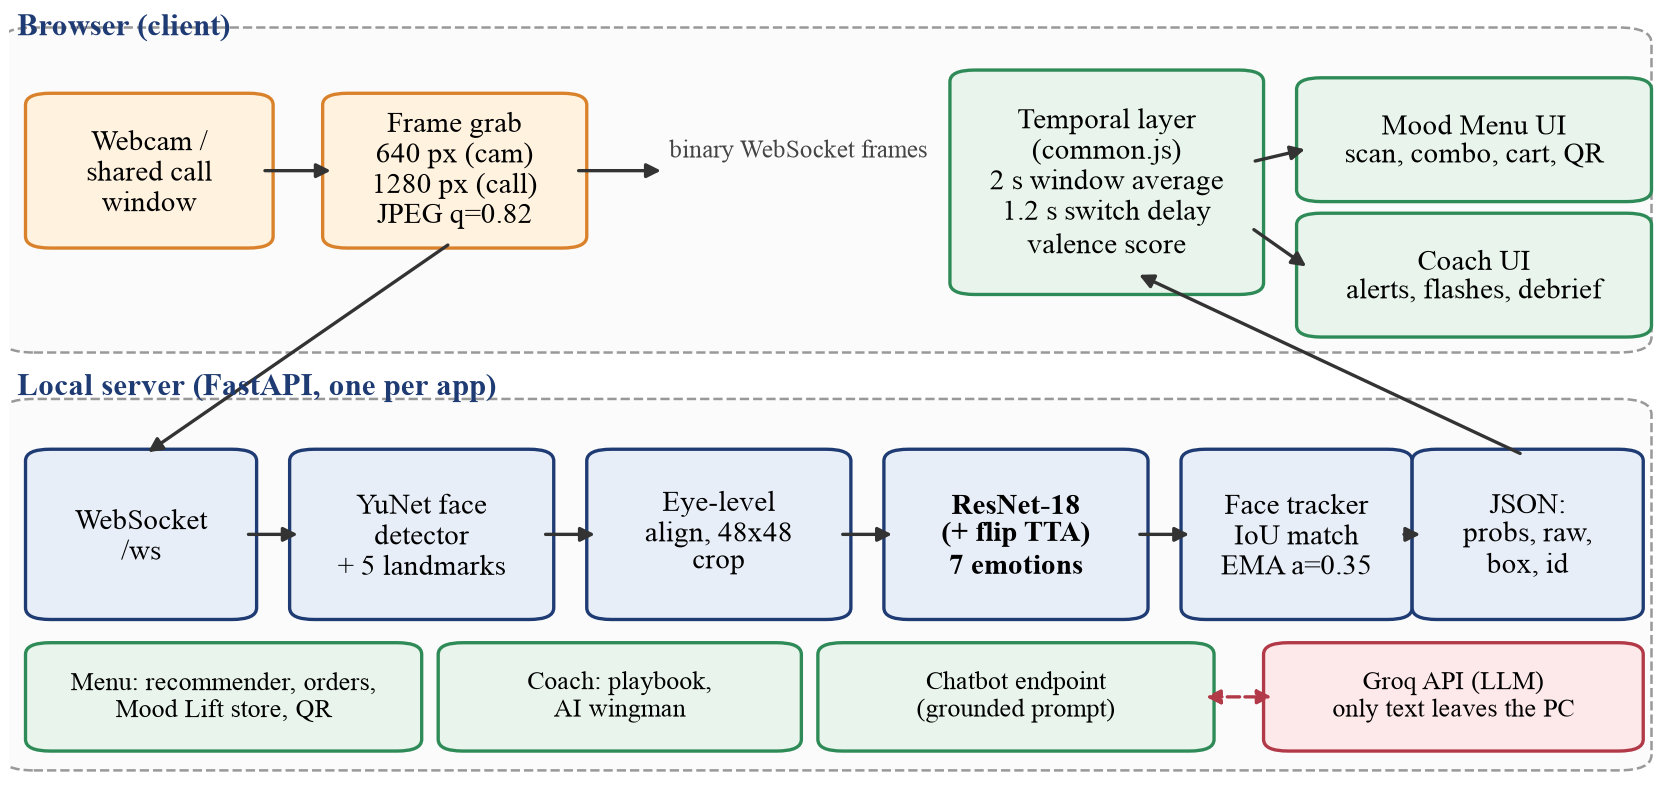
\includegraphics[width=0.88\textwidth]{fig_architecture.png}
\caption{Architecture used within both applications. The browser captures the camera frames and sends the JPEG buffers over a WebSocket to the FastAPI server. The server performs detection using YuNet, alignment to eye-level, and classification using the ResNet-18 classifier. The raw probabilities are smoothed using a temporal filter with hysteresis. The chatbots call the external LLM API.}
\label{fig:architecture}
\end{figure*}

\section{Expression Recognition Engine}
\subsection{Backbone and Training}
The classifier used is a ResNet-18~\cite{he}. This consists of a $7\times7$ convolution, 4 residual stages with 2 $3\times3$ convolutions each, global average pooling, dropout ($p=0.4$), and a 7-way linear layer. The $48\times48$ grayscale image is duplicated across 3 channels and scaled bilinearly to $112\times112$ to use pre-trained ImageNet weights.

The model was trained in 2 stages:

\subsubsection{Stage 1: FER-2013}
AdamW~\cite{adamw} was used with a learning rate of $10^{-3}$ and weight decay of 0.05. One-Cycle schedule~\cite{onecycle} was used for 40 epochs with a batch size of 128. The classes are unbalanced so the loss function was weighted for class $c$ as:
\begin{equation}
w_c = \sqrt{\frac{\max_{k} N_k}{N_c}}
\end{equation}
Where $N_c$ is the number of samples in class $c$ during training. Label smoothing~\cite{labelsmooth} was added with $\epsilon = 0.1$,
\begin{equation}
y_c^{\text{LS}} = (1 - \epsilon) y_c + \frac{\epsilon}{C},
\end{equation}
Mixup~\cite{mixup} was used ($\alpha = 0.2$) on half the mini-batch. Random Erasing~\cite{erasing} ($p=0.4$). Horizontal flips, rotations up to $\pm 12^\circ$, brightness and contrast was altered by up to $\pm 0.35$. During test time, the predictions were averaged from the original crop and mirrored crop.

\subsubsection{Stage 2: FER+ Soft Labels}
The model was fine-tuned on the vote counts for each class. If $v_c$ is the number of annotators that voted for class $c$ for an image then the target becomes:
\begin{equation}
q_c = \frac{v_c}{\sum_{k=1}^C v_k}.
\end{equation}
Kullback-Leibler divergence was used as the loss function with $q$ and the softmax output of the model $p$.
\begin{equation}
\mathcal{L}_{\text{KL}}(q, p) = \sum_{c=1}^C q_c \log \frac{q_c}{p_c} = \mathcal{H}(q, p) - \mathcal{H}(q).
\end{equation}
This ensures ambiguous faces (e.g. 60\% happy and 40\% surprise) are not forced into one class.

\subsection{Face Detection and Alignment}
The faces in the live frames are skewed and not centred, so the following processing is applied to each frame (Fig.~\ref{fig:pipeline}):
\begin{enumerate}
    \item \textbf{Detection.} The ONNX version of YuNet~\cite{yunet} is used to detect the face. This provides a bounding box $[x, y, w, h]$ and 5 facial landmarks (both eyes, nose tip, both mouth corners).
    \item \textbf{Alignment to eye level.} The skew is calculated using the line between the eyes. $p_L = (x_L, y_L)$ and $p_R = (x_R, y_R)$. Theta is calculated as:
    \begin{equation}
    \theta = \arctan2\left(\frac{y_R - y_L}{x_R - x_L}\right).
    \end{equation}
    The image is rotated about the midpoint $p_M = (p_L + p_R)/2$. The scaling is performed to ensure the distance between the eyes is fixed. This is done using the affine matrix:
    \begin{equation}
    M = \begin{bmatrix} s \cos\theta & -s \sin\theta & t_x \\ s \sin\theta & s \cos\theta & t_y \end{bmatrix}.
    \end{equation}
    The warped image is cropped, converted to grayscale and scaled to $48\times48$.
\end{enumerate}

\begin{figure*}[!t]
\centering
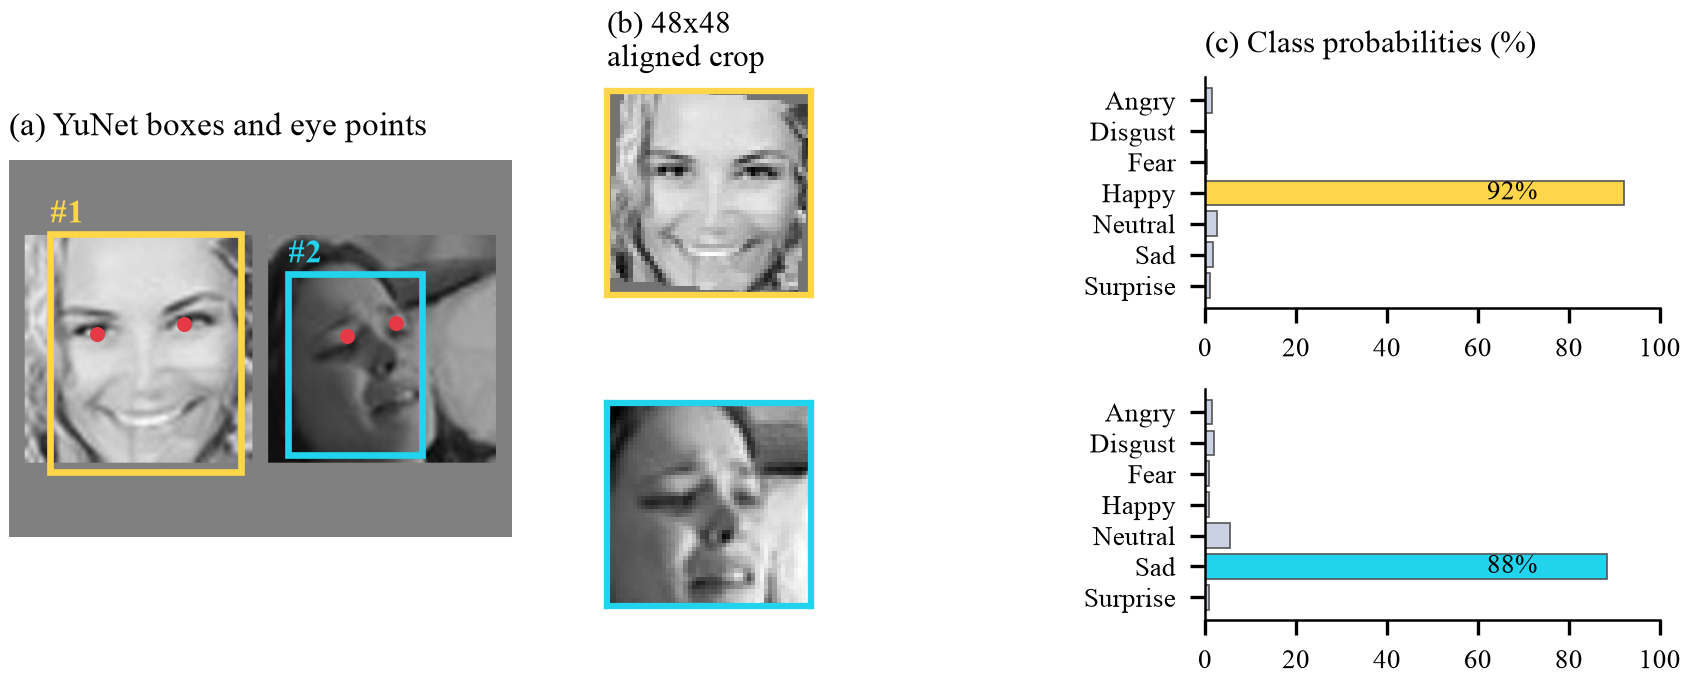
\includegraphics[width=0.88\textwidth]{fig_pipeline.png}
\caption{Face processing. (a) Camera frame with bounding boxes and landmarks from YuNet. (b) Aligned $48\times48$ grayscale crops using affine warp $M$. (c) Output of ResNet-18 softmax.}
\label{fig:pipeline}
\end{figure*}

\subsection{Temporal Smoothing and Hysteresis}
The predictions are very volatile for static faces. An EMA (exponential moving average) filter was applied. To prevent the label changing too frequently, a hysteresis rule was applied. The softmax vector at time $t$ ($p_t$) was filtered to get a smoothed vector ($s_t$):
\begin{equation}
s_t = \alpha p_t + (1 - \alpha) s_{t-1}, \qquad \alpha = 0.35.
\end{equation}
The label shown ($m_{t-1}$) was only updated to the best class ($c^*$) if:
\begin{equation}
s_t(c^*) \ge s_t(m_{t-1}) + \delta_{\text{hyst}} \quad \text{and} \quad \tau(c^*) \ge \tau_{\text{min}},
\end{equation}
where $\tau(c^*)$ is the time $c^*$ has been the top class, $\delta_{\text{hyst}} = 0.15$, $\tau_{\text{min}} = 1.2$\,s. These values were manually set based on watching the output on test videos. See Section~\ref{sec:results} for results.

\subsection{Micro-Expression Detection}
Micro-expressions are very quick movements in the face that can occur when the user is trying to hide their reaction. The system looks for a sudden increase in one of the classes. Let $s_t$ be the baseline probabilities (smoothed as above), and $p_t$ be the probabilities for the current frame. If there is a sudden increase in class $k$ (not the current baseline label) then:
\begin{equation}
p_t(k) - s_t(k) \ge \Delta_{\text{thresh}} \quad \text{and} \quad d_k \in [T_{\text{min}}, T_{\text{max}}],
\end{equation}
where $d_k$ is the time this excess has occurred for. $\Delta_{\text{thresh}} = 0.30$. $T_{\text{min}} = 140$\,ms (2 frames at 14\,fps) and $T_{\text{max}} = 650$\,ms (9 frames). Any change lasting longer than 650\,ms is considered a normal expression change.

\begin{table}[!t]
\centering
\caption{Alert Rules for Conversation Coach}
\label{tab:alerts}
\small
\begin{tabular}{@{}lll@{}}
\toprule
Alert & Trigger & Action \\
\midrule
Micro-expression & $\Delta p_k \ge 0.30$, $d \in [140, 650]$\,ms & Flash badge \\
Disengaged & Neutral $>0.70$ for $>4.0$\,s & ``Check in'' \\
Tension & Anger/Disgust $>0.45$ for $>2.0$\,s & ``De-escalate'' \\
Rapport & Happy $>0.60$, Positivity $> +25$ & ``Pacing good'' \\
No face & No face detected for $>4.0$\,s & ``Face lost'' \\
Group & $\ge 2$ faces for $>1.5$\,s & Room Mode \\
\bottomrule
\end{tabular}
\end{table}

\section{System Architecture}
Both applications used the same client-server architecture (Fig.~\ref{fig:architecture}). FastAPI~\cite{fastapi}, OpenCV~\cite{opencv}, and PyTorch~\cite{pytorch} were used. The video is captured using \texttt{getUserMedia} and is $640\times480$ resolution. The JPEG frames are sent over a WebSocket at $\sim$14\,fps.

\subsection{Concurrent Processing}
Neural network inference can be slow when multiple tabs/users are streaming. We found the inference slowed down when using the unified memory GPU (Apple Silicon -- Metal Performance Shaders (MPS)). We use an \texttt{asyncio} lock around the model call to ensure only one forward pass is run at a time. The JPEG decoding, tracking and post-processing is run on a thread pool. This kept the processing time below 25\,ms for multiple clients.

\subsection{Privacy}
All processing is done on the host device. No video frames, face crops or embeddings are saved to disk. No data is sent to a remote server. The only data sent is text relating to the detected emotion label, positivity score and chat messages from the user to the LLM service.

\section{Application 1: Smash Guys Mood Menu}
\subsection{Recommender}
The inputs to the recommender are the detected mood ($m=1,\dots,7$), diet setting ($D \in \{\text{Any}, \text{Veg}, \text{NonVeg}\}$), spice limit ($S \in \{0, 1, 2\}$), allergens to avoid ($\mathcal{A}_{\text{avoid}}$) and budget ($B$). The recommender selects one item from each course ($c = \{d_{\text{main}}, d_{\text{side}}, d_{\text{drink}}, d_{\text{dessert}}\}$) from the menu ($\mathcal{M}$). The $\text{Affinity}(d, m)$ is manually set based on the flavour tags of the dish (e.g. comforting umami for sadness, bright citrus for tiredness, indulgent for happiness). $\Delta_{\text{lift}}(d)$ is the average Mood Lift recorded for the dish so far. The function to maximise is:
\begin{equation}
\max_{c \subseteq \mathcal{M}} \sum_{d \in c} \left( w_{\text{aff}} \cdot \text{Affinity}(d, m) + w_{\text{lift}} \cdot \Delta_{\text{lift}}(d) + \epsilon_d \right)
\end{equation}
subject to:
\begin{align}
|c \cap \mathcal{M}_{\text{course}}| &= 1 \quad \forall \text{course} \in \{\text{main}, \text{side}, \text{drink}, \text{dessert}\} \\
\text{Diet}(d) &= D \quad \text{if } D \neq \text{Any} \\
\text{Spice}(d) &\le S \\
\text{Allergens}(d) \cap \mathcal{A}_{\text{avoid}} &= \emptyset \\
\sum_{d \in c} \text{Price}(d) &\le B.
\end{align}
The $\epsilon_d \sim \mathcal{N}(0, \sigma^2)$ is a small amount of random noise added to make the combinations different when the shuffle is repeated. If the budget is too low for 4 courses then courses are removed starting with the dessert, side, drink. The main course will always remain.

\subsection{Mood Lift Rescan}
We wanted to allow the user to check if they had a better expression after eating the recommended food. The process is:
\begin{enumerate}
    \item \textbf{Before Eating.} During the scanning process for ordering the positivity score ($P_{\text{pre}}$) is recorded. $P_{\text{pre}} \in [-100, +100]$.
    \item \textbf{After Eating.} The diner opens their digital order ticket and starts the rescan. This gives a positivity score ($P_{\text{post}}$).
    \item \textbf{Update.} Calculate the difference in positivity ($\Delta P$) and update the lift stored for each dish in the order. This uses a moving average:
    \begin{equation}
    \Delta_{\text{lift}}^{(t)}(d) = (1 - \beta) \Delta_{\text{lift}}^{(t-1)}(d) + \beta \Delta P.
    \end{equation}
\end{enumerate}
This means dishes with a higher positivity after will be ranked higher. We have not yet gathered enough rescans to determine if this is an indication of the food. (See Section~\ref{sec:limits}).

\subsection{Table Mode and Chatbot}
If multiple faces are detected then Table Mode will track each diner. Each diner has their own card. The chatbot (Smashy) receives the full menu, current prices, filters and diner's mood. When recommending a dish it will include the item tag ($[\#\text{ID}]$). This is turned into an Add to Cart button within the interface.

\section{Application 2: Live Conversation Coach}
The Coach provides feedback on the expressions of the conversation partner during professional, social and personal conversations.

\subsection{Positivity Index}
The 7 class probabilities are combined into one score ($P(t) \in [-100, +100]$):
\begin{equation}
P(t) = 100 \cdot \sum_{c=1}^C v_c \cdot s_t(c),
\end{equation}
where $v = [+1.0, -0.6, -0.7, -0.8, +0.4, 0.0, -0.7]$ for classes [happy, sad, angry, fear, surprise, neutral, disgust]. These were manually selected. This drives the gauge and short advice (e.g. ``Pacing is ideal'', ``Check in on hesitancy'').

\subsection{Sentence Scoring}
The Web Speech Recognition API is used within the browser to capture what the speaker is saying. For each completed sentence ($[t_{\text{start}}, t_{\text{end}}]$) the average positivity of the listener is calculated for the 3 seconds before the sentence, and the window starting 1 second after the end of the sentence (3 seconds). This allows for reaction time:
\begin{equation}
\Delta P_{\text{reaction}} = \bar{P}[t_{\text{end}}+1, t_{\text{end}}+4] - \bar{P}[t_{\text{start}}-3, t_{\text{start}}].
\end{equation}
If the change in positivity is $\ge +10$ then sentence is labelled as ``Landed well''. If the change in positivity is $\le -10$ then sentence is labelled as ``Hit a nerve''. This only indicates a change in the listener's expression, it does not indicate that the sentence caused the change.

\subsection{Room Mode and Debrief}
If there are two or more faces, Room Mode can be activated to show one card per person. A label will appear that tells you the overall mood of the room (Buzzing, Warm, Flat or Tense). At the end of the session, a downloadable report is provided that tells you how long the session lasted along with some statistics on how positive the session was. There is also a chart showing how positive the session was along with the micro-expression flags. Finally, there are a few suggestions.

\section{Experimental Setup}
All experiments were run on one Apple MacBook (M2 computer with 8 CPU cores, 10 GPU cores and 16\,GB of memory), running macOS (v15.4.1). Python (v3.12), PyTorch (v2.14 MPS), OpenCV (v4.14) and FastAPI (v0.162) were used.

We ran the following evaluations:
\begin{itemize}
    \item \textbf{Classification.} Top 1 accuracy and macro-F1 were calculated for two datasets. The FER-2013 Test dataset contained 7,178 images, whilst the FER+ PrivateTest dataset contained 3,519 images. A mirrored average was used.
    \item \textbf{Camera Pipeline.} YuNet detection and alignment process was run on all 6,970 faces in the FER-2013 Test dataset.
    \item \textbf{Latency.} 200 consecutive frames were collected after 30 warm-up frames. Decoding, detection, alignment, classification and WebSocket latency times were collected.
    \item \textbf{Temporal Stability.} A total of 280 videos were created containing stable faces with a speed of 14\,fps. Landmark jittering was applied using Gaussian. How many times the label changed, how long the delay was and how many flashes could be captured in these simulated videos (between 70--850\,ms).
    \item \textbf{Stress Test (Recommender).} A total of 3,000 random requests were made for the diners containing a variety of constraints.
    \item \textbf{Chatbot and Browser.} 22 prompts were created for the chatbots. 28 tests were created to test the UI using headless browsers.
\end{itemize}

\section{Demonstration Sessions}
Both applications were run using a live webcam and some screenshots were recorded. See Fig.~\ref{fig:real_menu} and Fig.~\ref{fig:real_coach}. This is just an example of how the applications work.

\subsection{Mood Menu}
Fig.~\ref{fig:real_menu} shows an example of an ordering session:
\begin{enumerate}
    \item \textbf{Scan (Fig.~\ref{fig:real_menu}a).} The diner faces the webcam with normal lighting in the room. The system recognises the diner is happy (86.4\% confidence). Four course recommendation was suggested (OG Smash burger, Cajun Fries, Cold Chocolate, Classic Cheesecake).
    \item \textbf{Filters (Fig.~\ref{fig:real_menu}b).} The diner selects Vegetarian and Medium spiciness. Nuts and Alcohol were also excluded. The solver recomputed the recommendation in less than 2\,ms. A vegetarian recommendation that met all of the constraints was provided.
    \item \textbf{Chat (Fig.~\ref{fig:real_menu}c).} The diner asks Smashy, ``What burger should I get?'' The recommendation uses the detected mood. OG Smash was suggested. Buttons were added to help add items to the cart ($[\#\text{ID}]$).
    \item \textbf{Mood Lift (Fig.~\ref{fig:real_menu}d).} After the meal, the diner initiates the rescan. The positivity score had increased by 18. The lift values for the dishes ordered had been updated.
\end{enumerate}

\begin{figure*}[!t]
\centering
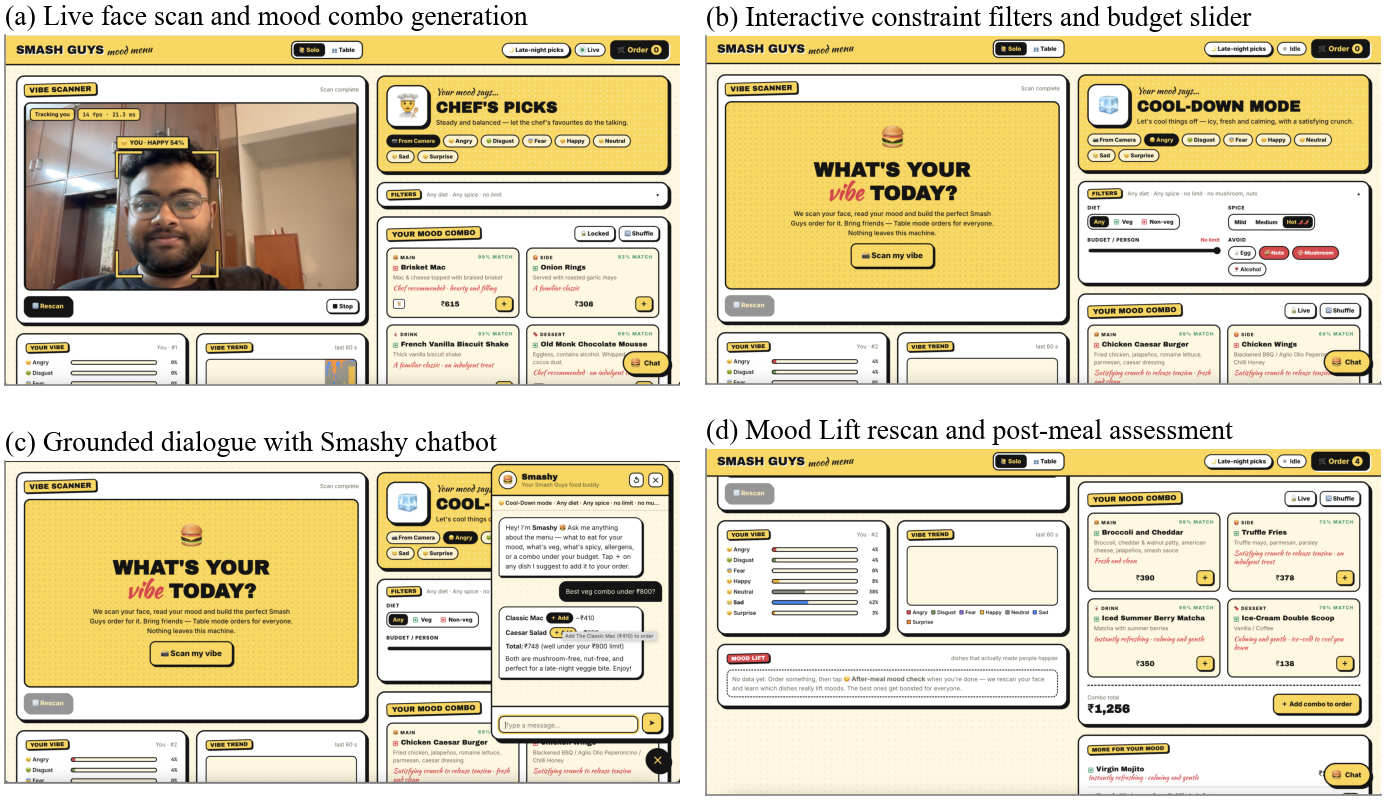
\includegraphics[width=0.92\textwidth]{fig_real_menu.png}
\caption{Smash Guys Mood Menu with a live webcam: (a) Scanning the face using bounding box. Emotion, confidence and recommendation. (b) Filters panel for changing the diet, spiciness, budget and allergens. (c) Chat with Smashy and Add To Cart buttons. (d) Mood Lift with rescan.}
\label{fig:real_menu}
\end{figure*}

\subsection{Conversation Coach}
Fig.~\ref{fig:real_coach} shows an example of a 15\,min professional conversation.
\begin{enumerate}
    \item \textbf{Live Feedback (Fig.~\ref{fig:real_coach}a).} The system tracks the partner's face and displays their current emotion. The positivity value was $+45$. Advice was given by stating ``Pacing is good --- Continue to elaborate on this topic''.
    \item \textbf{Micro-expression (Fig.~\ref{fig:real_coach}b).} During the negotiation, something unexpected was said. The listener expressed their surprise and scepticism via a 320\,ms flash. An alert was triggered and the advice changed to ``Check for any hesitation''.
    \item \textbf{AI Wingman (Fig.~\ref{fig:real_coach}c).} The user asks the Wingman chatbot how to phrase their response. The bot knows the context of the conversation along with the history of the mood and last few lines of the transcript. A suggestion is given for how to phrase the response without trying to manipulate the other person.
    \item \textbf{Debrief (Fig.~\ref{fig:real_coach}d).} After the conversation, a report was produced. An emotion timeline was provided along with the sentences with the highest positivity and negativity. Suggestions were given for future meetings.
\end{enumerate}

\begin{figure*}[!t]
\centering
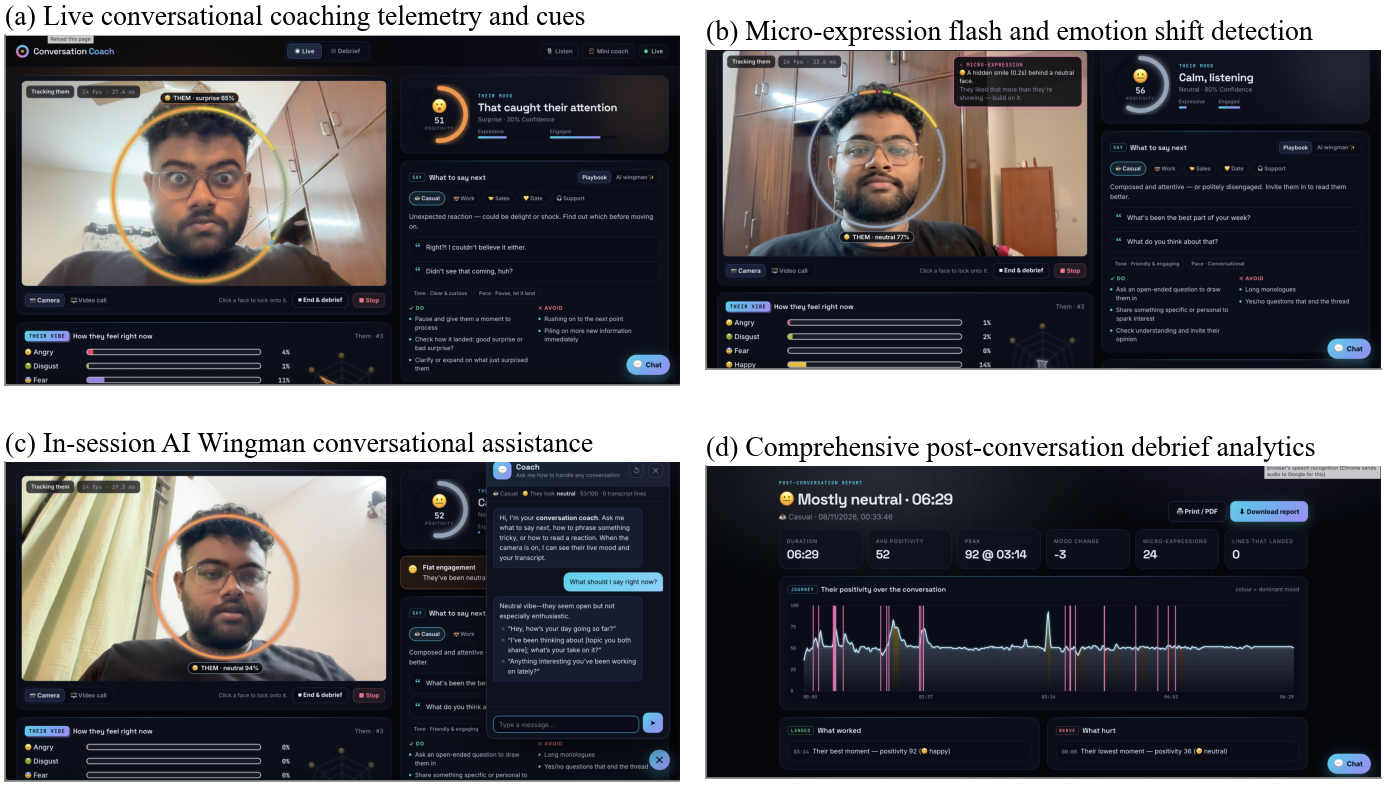
\includegraphics[width=0.92\textwidth]{fig_real_coach.png}
\caption{Conversation Coach in a live conversation: (a) Tracking face with emotion, positivity and advice. (b) Micro-expression alert. (c) AI Wingman chat. (d) Debrief after the session including positivity chart and scored sentences.}
\label{fig:real_coach}
\end{figure*}

\section{Results}
\label{sec:results}
\subsection{Classification Accuracy and Checkpoint Selection}
The results can be seen in Table~\ref{tab:models}. ResNet-18 achieves 69.99\% accuracy on FER-2013. This is 5.74\% higher than the custom CNN. The model was then fine tuned with the soft labels from FER+. This boosted the accuracy to 85.08\% on PrivateTest with a macro-F1 of 0.766.

The most accurate checkpoint was not selected due to it performing well on the common classes only. This can be seen in Fig.~\ref{fig:f1}. The model performs badly on the rarer classes. The disgust class had a recall of only 53.6\% and the fear class had a recall of 44.8\%. The checkpoint chosen had an accuracy of 83.38\% (1.7\% less accurate than the most accurate checkpoint). However, the rare classes had a much higher recall. Disgust had a recall of 78.6\% and Fear had a recall of 69.8\% (25.0\% higher). The checkpoint also performed 2.2\% better on the camera aligned crops. Happiness, surprise and neutral had a high F1 score ($>$84\%) on FER+. The main issues were with fear, surprise and sadness. The accuracy dropped by 2.8\% due to the test faces going through the YuNet pipeline rather than the provided crops.

\begin{table*}[!t]
\centering
\caption{Classifier Comparison on FER-2013 and FER+}
\label{tab:models}
\small
\begin{tabular}{@{}lrrrrr@{}}
\toprule
Model & Params (M) & FER-2013 Acc (\%) & FER-2013 Macro-F1 & FER+ Acc (\%) & FER+ Macro-F1 \\
\midrule
Custom CNN (4 conv blocks) & 1.24 & 64.25 & 0.611 & -- & -- \\
ResNet-18 (Stage 1) & 11.18 & \textbf{69.99} & \textbf{0.690} & 64.59 & 0.573 \\
ResNet-34 (Stage 1, aligned crops) & 21.30 & 69.91 & 0.684 & -- & -- \\
ResNet-18 (Stage 2, best-accuracy checkpoint) & 11.18 & 60.99 & 0.543 & \textbf{85.08} & \textbf{0.766} \\
\textbf{ResNet-18 (Stage 2, shipped checkpoint)} & 11.18 & 63.23 & 0.584 & 83.38 & 0.755 \\
\bottomrule
\end{tabular}
\end{table*}

\begin{figure*}[!t]
\centering
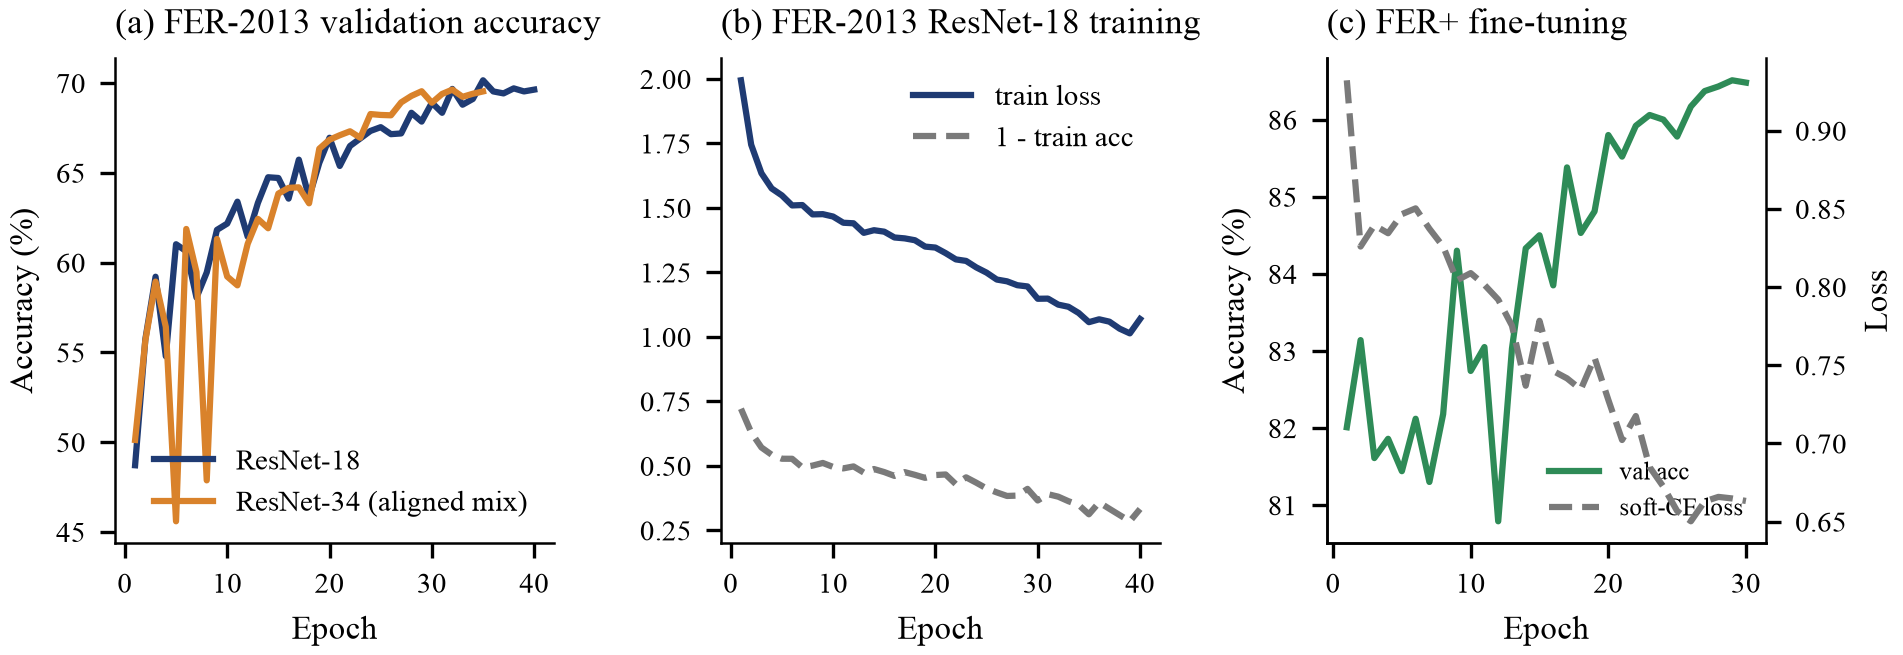
\includegraphics[width=0.88\textwidth]{fig_training.png}
\caption{Training curves: (a) FER-2013 validation accuracy over 40 epochs; (b) training loss and training error with label smoothing and mixup; (c) FER+ fine-tuning, showing validation accuracy and KL loss.}
\label{fig:training}
\end{figure*}

\begin{figure}[!t]
\centering
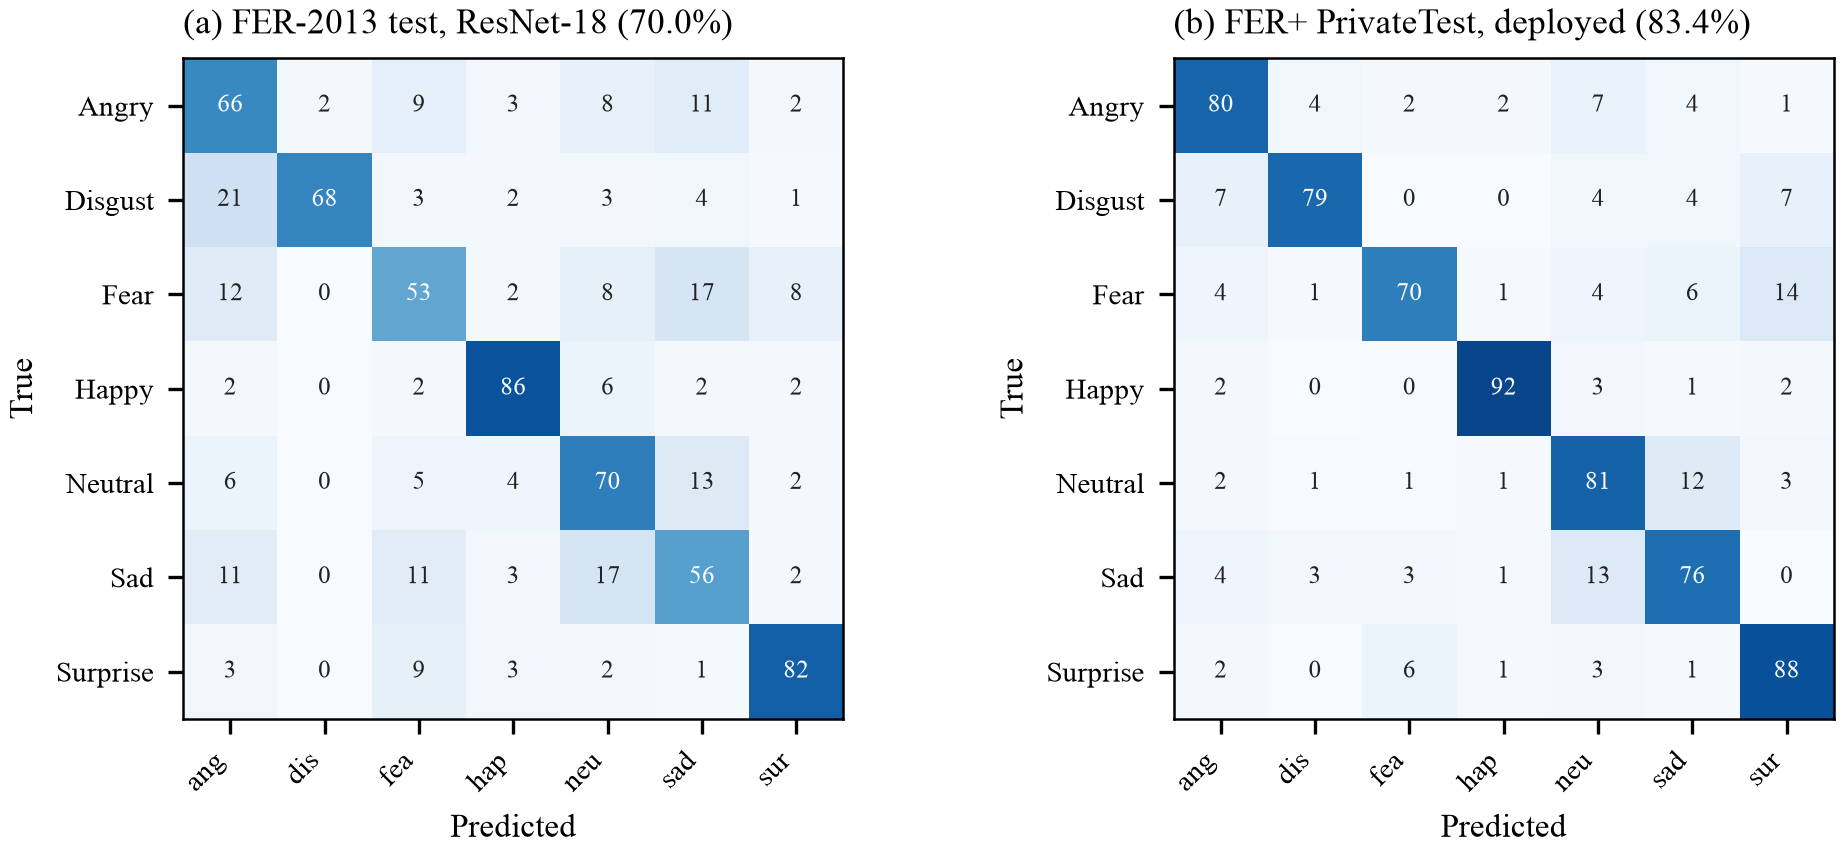
\includegraphics[width=0.95\columnwidth]{fig_confusion.png}
\caption{Confusion matrices (\%): (a) Stage 1 ResNet-18 on the FER-2013 test set; (b) shipped Stage 2 ResNet-18 on FER+ PrivateTest.}
\label{fig:confusion}
\end{figure}

\begin{figure}[!t]
\centering
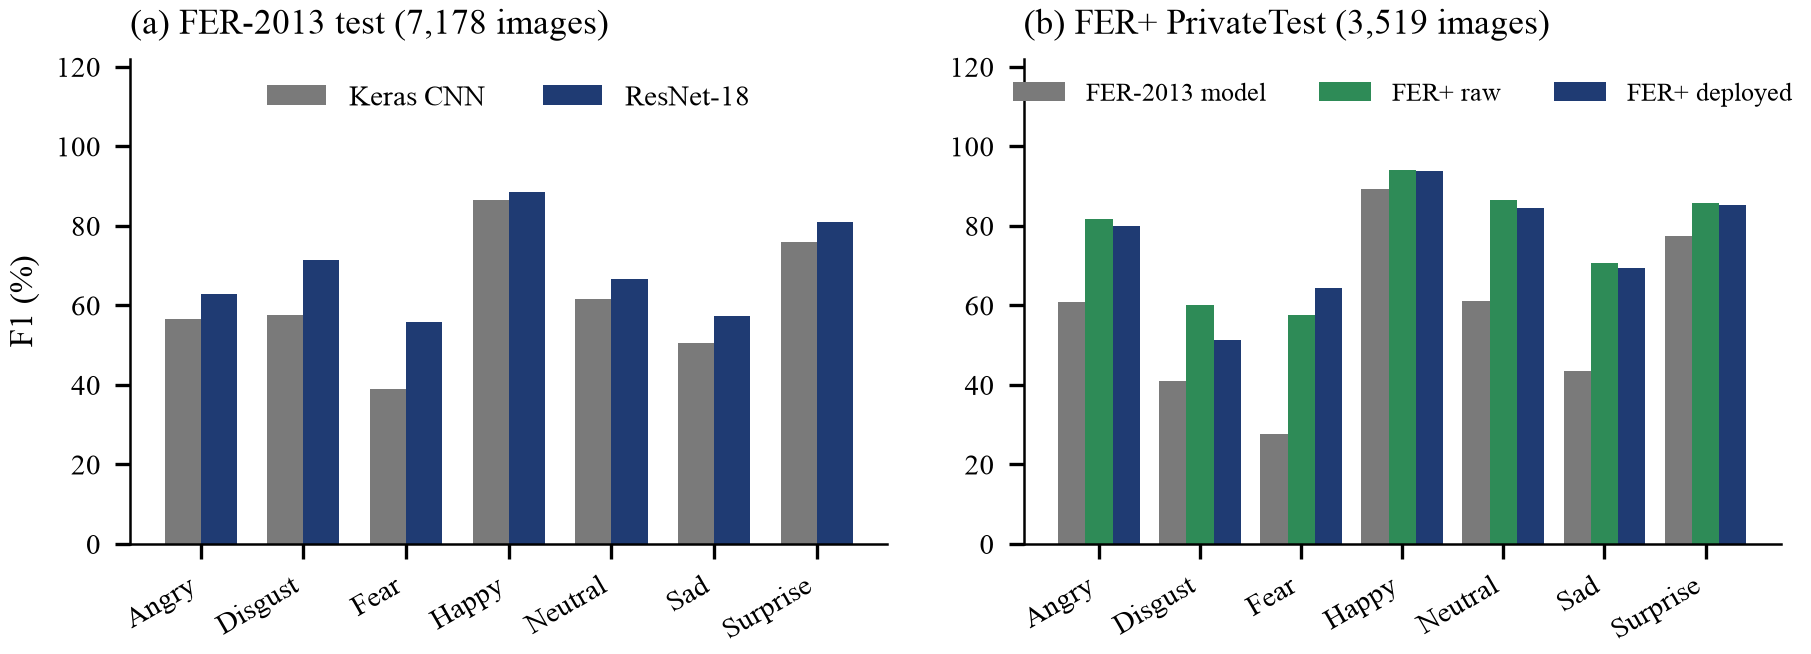
\includegraphics[width=0.95\columnwidth]{fig_f1.png}
\caption{Per-class F1: (a) Stage 1 model on FER-2013; (b) FER+ checkpoints, showing that the shipped model recalls more of the rare classes (disgust and fear).}
\label{fig:f1}
\end{figure}

\subsection{Latency}
The latency for different sizes and numbers of faces can be seen in Table~\ref{tab:latency} and Fig.~\ref{fig:latency}. Using one face with a size of $640\times480$:
\begin{itemize}
    \item JPEG Decode -- 0.9\,ms
    \item YuNet Detection and Landmarks -- 12.1\,ms
    \item Aligning and Normalising -- 0.4\,ms
    \item ResNet-18 Forward Pass (MPS) -- 9.6\,ms
    \item Total Time per Frame -- 22.6\,ms (approx 44\,fps).
\end{itemize}
With two faces the total time was 28.6\,ms and 31.6\,ms with four faces. This was well within the 71.4\,ms available at 14\,fps.

On average the WebSocket latency was 30.0\,ms (95th percentile: 36.4\,ms) for Mood Menu and 32.6\,ms (95th percentile: 42.5\,ms) for Conversation Coach.

\begin{figure}[!t]
\centering
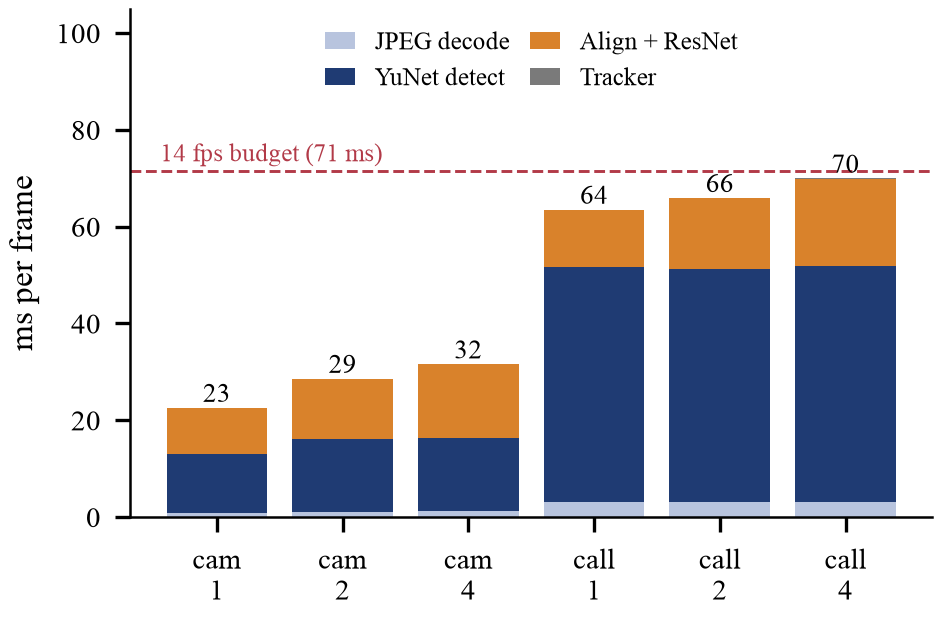
\includegraphics[width=0.92\columnwidth]{fig_latency.png}
\caption{Server time per frame for different face counts and resolutions on the M2. The dashed line is the 71.4\,ms budget at 14\,fps.}
\label{fig:latency}
\end{figure}

\begin{table}[!t]
\centering
\caption{Latency by Resolution and Face Count}
\label{tab:latency}
\small
\begin{tabular}{@{}lrrrr@{}}
\toprule
Resolution & Faces & Detection (ms) & Inference (ms) & Total (ms) \\
\midrule
$640\times480$ & 1 & 12.1 & 9.6 & 22.6 \\
$640\times480$ & 2 & 14.8 & 12.4 & 28.6 \\
$640\times480$ & 4 & 16.2 & 14.1 & 31.6 \\
$1280\times720$ & 1 & 48.2 & 9.7 & 59.4 \\
$1280\times720$ & 2 & 51.4 & 12.6 & 65.5 \\
$1280\times720$ & 4 & 54.1 & 14.3 & 69.8 \\
\bottomrule
\end{tabular}
\end{table}

\subsection{Temporal Smoothing}
The results from the 280 simulated stable face sequences can be seen in Fig.~\ref{fig:temporal}:
\begin{itemize}
    \item \textbf{Flickering (Fig.~\ref{fig:temporal}a).} On average there were 14.2 changes between each label per 10 seconds. However when EMA was applied ($\alpha = 0.35$) this decreased to 3.7 changes. Adding hysteresis reduced this to 0.1 (99.3\% decrease).
    \item \textbf{Delay (Fig.~\ref{fig:temporal}b).} The time taken for a label to change after a genuine change was a median of 2.36 seconds (90th percentile: 2.50 seconds). This was observed over 210 changes.
    \item \textbf{Micro-expressions (Fig.~\ref{fig:temporal}c).} 94\% of the simulated flashes (140--650\,ms) were detected on a happy baselined sequence. 97\% were detected on a neutral baselined sequence. All single frame noise (70\,ms) were ignored. Changes longer than 700\,ms were treated like normal expression changes. Only 6 false alarms were raised over the 45 minutes of stable faces (0.13 per minute).
\end{itemize}
The results above are from simulated flashes and jittered videos. This shows how the algorithm works but does not show how well it detects micro-expressions on people.

\begin{figure*}[!t]
\centering
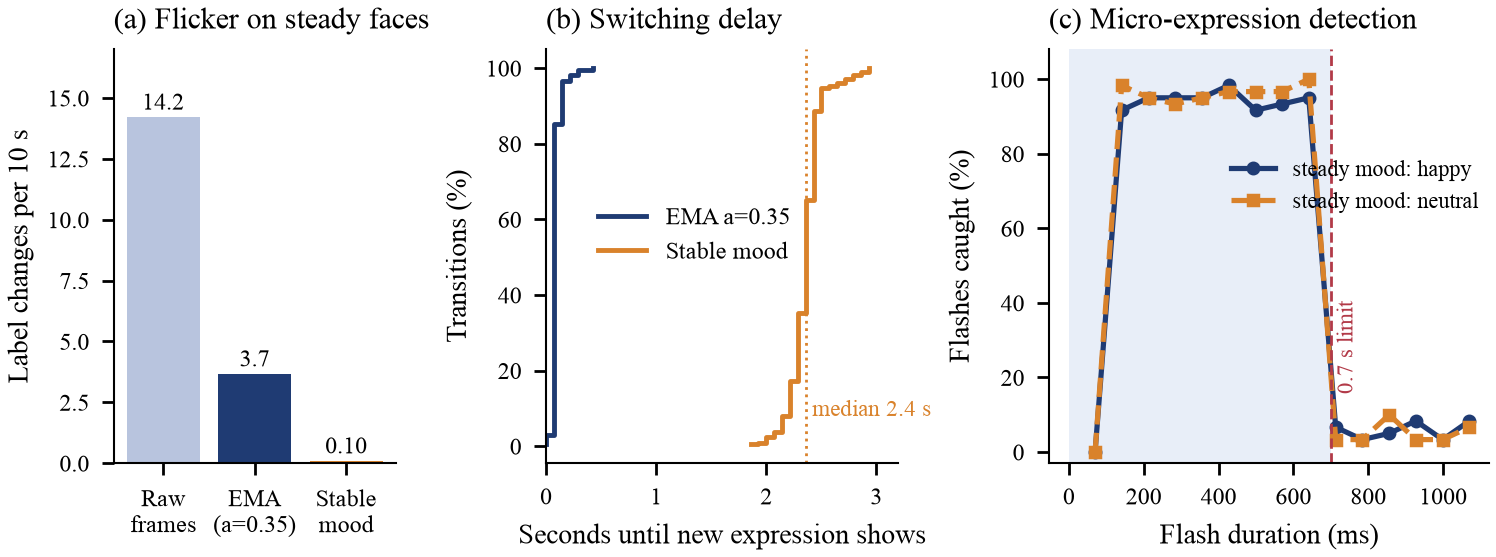
\includegraphics[width=0.88\textwidth]{fig_temporal.png}
\caption{Temporal behavior: (a) label changes on steady faces fall from 14.2 to 0.1 per 10\,s; (b) cumulative distribution of switching delay (median 2.36\,s); (c) detection rate against flash duration.}
\label{fig:temporal}
\end{figure*}

\subsection{Recommender Testing}
3,000 random tests were run with a variety of moods, diets, spicy levels and budgets.
\begin{itemize}
    \item \textbf{Constraints.} No violations of the diet, allergens, spicy level or budget.
    \item \textbf{Mood Match (Fig.~\ref{fig:rec}a).} 100\% of the recommended dishes had the required tag for 5 moods. 75\% for surprise and 50\% for angry. Randomly choosing had a much lower percentage (16--61\%). 0\% of the recommended combinations had the tag that should be avoided by the mood. Up to 42\% of random combinations had this tag.
    \item \textbf{Diversity (Fig.~\ref{fig:rec}b).} 4--14 unique combinations were found using 100 random seeds for each mood. Each new combination replaced all of the previous dishes when 700 Shuffle buttons were pressed.
\end{itemize}
The moods used for scoring are the same as those being optimised by the recommender. This proves that the optimiser is using its own scoring system. It does not tell us if the diners actually like the recommendations.

\begin{figure}[!t]
\centering
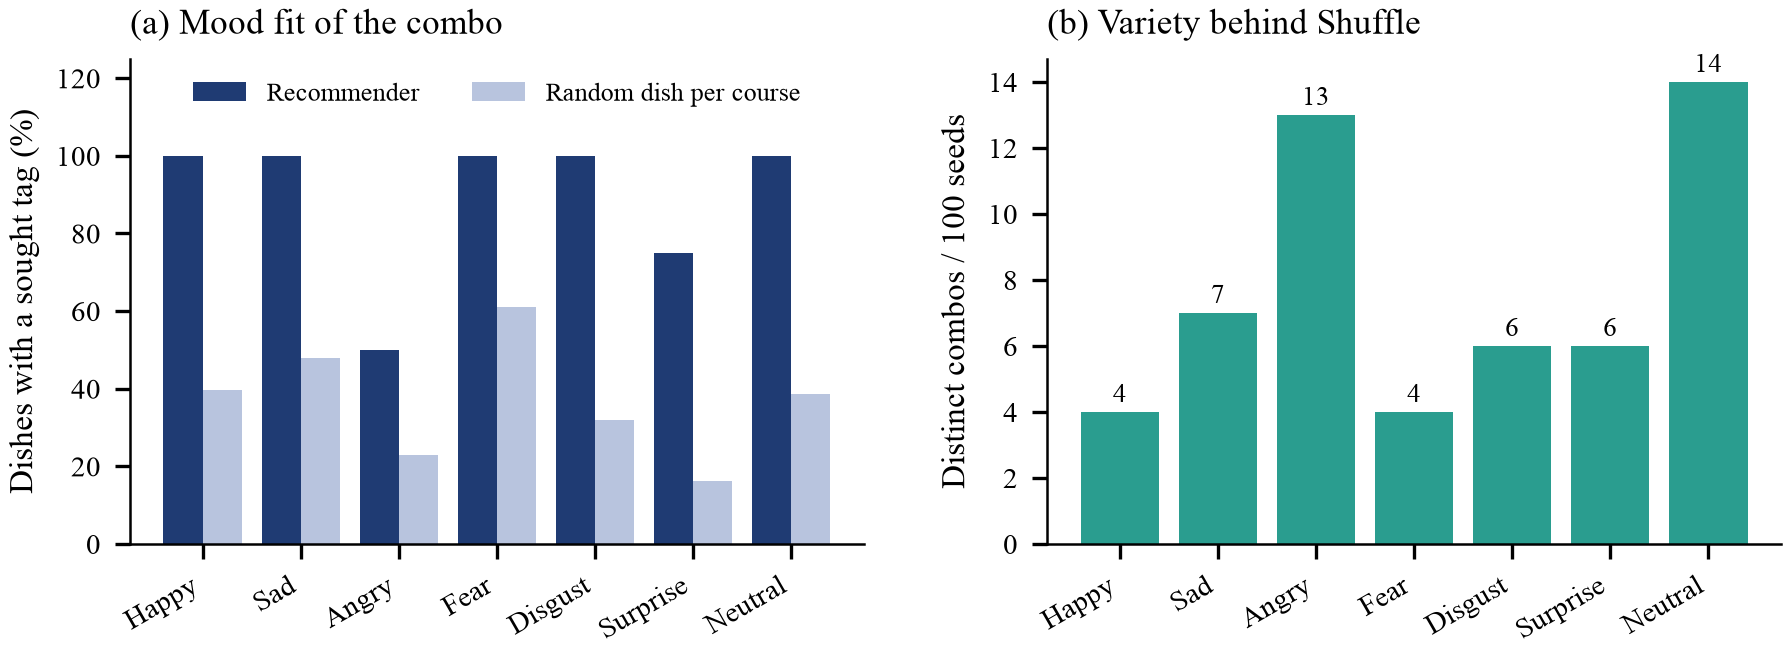
\includegraphics[width=0.92\columnwidth]{fig_recommender.png}
\caption{Recommender tests: (a) share of recommended dishes with mood-sought tags, compared with random choice; (b) number of distinct combinations across seeds.}
\label{fig:rec}
\end{figure}

\subsection{Chatbot Testing}
22 prompts were created (12 for the menu bot and 10 for the coach) and sent to Groq's \texttt{gpt-oss-120b}.
\begin{itemize}
    \item \textbf{Smashy.} 11/12 tests passed on first attempt. There was an issue with the test script regex causing it to fail. Once fixed the bot did not mention any dishes not on the menu. It respected the allergen filters and had the correct $[\#\text{ID}]$ tags.
    \item \textbf{Coach Bot.} All 10 tests passed across 5 conversation settings. The bot refused to provide manipulative social tactics.
    \item \textbf{Speed.} The median time taken for responses was 741\,ms for Smashy and 744\,ms for the coach (Table~\ref{tab:chat}).
\end{itemize}

\begin{table}[!t]
\centering
\caption{Chatbot Test Results (after fixing the test-script bug)}
\label{tab:chat}
\small
\begin{tabular}{@{}lrrrr@{}}
\toprule
Chatbot & Cases & Passed & Pass rate (\%) & Median latency \\
\midrule
Smashy (menu) & 12 & 12 & 100.0 & 741\,ms \\
Conversation Coach & 10 & 10 & 100.0 & 744\,ms \\
\bottomrule
\end{tabular}
\end{table}

\begin{figure}[!t]
\centering
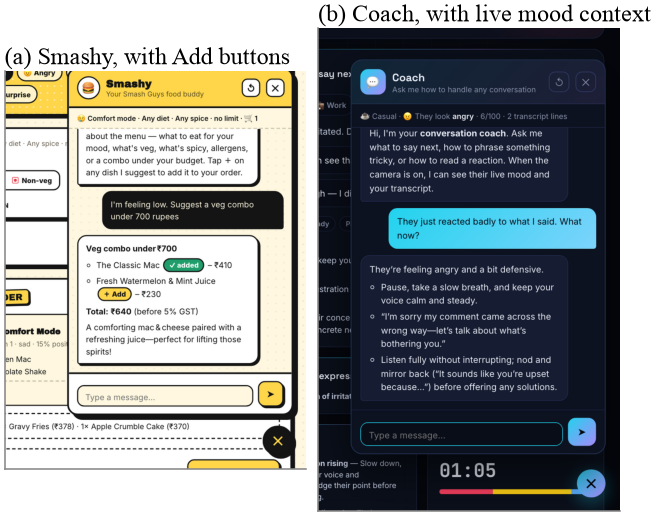
\includegraphics[width=0.85\columnwidth]{fig_ui_chat.png}
\caption{Chat interfaces: (a) Smashy recommending dishes with ``Add to Cart'' buttons; (b) the coach giving advice based on the listener's current mood.}
\label{fig:uichat}
\end{figure}

\subsection{Automated Browser Testing}
A script was run to test the headless Chromium browser. A virtual camera was used and 28 tests were completed.
\begin{itemize}
    \item \textbf{Mood Menu (15 tests).} Face detection, Diet filter, Spicy limit, Allergen block, Budget slider, Shuffle diversity, Course lock, GST calculation, Bill split, QR ticket, Mood Lift pop-up, Digital receipt, Table Mode tracking and Add to cart from chat.
    \item \textbf{Conversation Coach (13 tests).} Live emotion tracking, Advice, Settings change, Alerts, Transcript scoring, Micro-expression detection, Table Mode, Wingman responses, Audio selection and Debrief report.
\end{itemize}
All 28 tests passed and no errors were shown in the browser console. This shows that the features work but does not show how useful they are.

\section{Discussion}
\subsection{What We Have Learnt}
\begin{itemize}
    \item \textbf{Grounded Prompts.} The menu bot would sometimes mention side dishes and drinks that were not on the menu. By including the whole menu (72 items) and allergen tags in the system prompt, no made-up items were mentioned during testing.
    \item \textbf{Accuracy was not the priority.} The most accurate checkpoint did not provide good results for disgust and fear. Instead, a model with better recall for the rare classes was chosen. The model also had better results for the aligned crops.
    \item \textbf{Trade-off between stability and delay.} The raw labels were too unstable to read. However increasing the smoothing caused the labels to be slower to update with real changes. Using $\alpha = 0.35$ and $\delta_{\text{hyst}} = 0.15$ gave a median delay of approx 2.3 seconds. This was considered to be acceptable by observing the output.
\end{itemize}

\subsection{Limitations}
\label{sec:limits}
\begin{itemize}
    \item \textbf{Camera and Lighting.} The eye alignment helps with the head tilt. However during low lighting, the webcam has more noise and the landmarks from YuNet are less accurate.
    \item \textbf{Speaker Separation.} The Coach only transcribes what the speaker is saying. If there are multiple people in conversation, the user has to manually switch between speakers. No speaker diarisation is used.
    \item \textbf{No User Study.} The tests show the software works as intended. However we have not measured how useful the advice is to users. We have not measured if diners enjoyed the recommendations. We have not measured if Mood Lift is providing information about the food or just the diner's general mood and how much time has passed. The micro-expression detector was only tested with simulated flashes. We have not tested it with labelled micro-expression data.
    \item \textbf{Self-designed tests.} The recommender, chatbot and browser tests were self-designed. Assumptions have been made in the code.
\end{itemize}

\section{Ethics}
\begin{itemize}
    \item \textbf{Expressions not feelings.} As mentioned by Barrett et al.~\cite{barrett}, the applications do not provide a diagnosis but instead provide behavioural cues.
    \item \textbf{Local processing.} No video, face crops or landmark coordinates were stored or sent over the network. However text (such as emotion, positivity and chat) was sent to the LLM service.
    \item \textbf{Intended use.} The tools were intended to provide personal coaching and recommendations for dining. There are no features for covert monitoring, employee productivity, exam proctoring or hiring decisions. We would not recommend using these tools for these purposes.
\end{itemize}

\section{Conclusion}
MoodLens demonstrates how a ResNet-18 expression classifier can be implemented into two interactive web applications. Using eye alignment, exponential smoothing with hysteresis, constrained menu recommender, micro-expression detection and grounded prompts for chatbots. The applications can run in real time on a laptop. With 1--4 faces ($640\times480$), the applications take approximately 23--32\,ms per frame. The applications need to be tested with real users. The micro-expression detection needs to be tested with labelled data. We also need to check if Mood Lift provides an effect from the food.

%%BIB%%

\end{document}
